\chapter{Faster Queries using an Inverted Index}

\section{Task}
When using a search engine, the most important aspect is to be able to perform a search and get the results almost instantaneously. One way of doing this is by using an {\tt InvertedIndex}, which sorts the websites according to the words contained in each website. Hence when searching for a specific term, instead of going over every word contained in every website, it will retrieve websites mapped to the search term. While building the {\tt InvertedIndex} can be system heavy, it is a one time operation that will allow the search engine to answer queries significantly faster.

\section{Basic Approach}
All the files regarding the classes mentioned on this chapter can be found on the folder src/main/java/searchengine.\\
The {\tt Index} was generalised into an interface to make it easy to test the different indices and switch between them. The following methods define the aforementioned {\tt Index} interface:
\begin{itemize}
    \item {\tt build} — Processes a list of websites into the data structure.
    \item {\tt lookup} — Given a query {\tt String}, returns a list of all websites that contain the query.
    \item {\tt provideIndex} — Provides all websites in a given {\tt Index} as a collection.
\end{itemize}
The inverted indices were then implemented using inheritance, since both the {\tt InvertedIndexHashMap} and {\tt InvertedIndexTreeMap} can be given exactly the same methods, the only difference being their individual data structure.

\section{Technical Description}
As previously stated, a generalised {\tt Index} interface was created. Each of the classes below implements this interface, visualised in \ref{fig:Index:uml}.

\begin{figure}[!h]
    \centering
    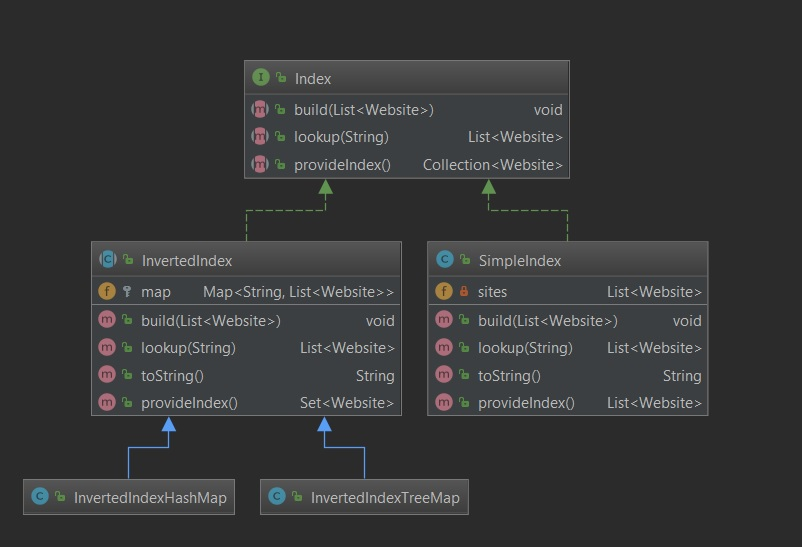
\includegraphics[width=\textwidth]{figures/Diagram_InvertedIndices}
    \caption{UML Diagram for the Software Architecture of Index data structures.}
    \label{fig:Index:uml}
\end{figure}

\subsection{{\tt SimpleIndex}}
The provided default way of indexing data was called {\tt SimpleIndex}. The {\tt build} method simply takes a list of websites and stores it in its {\tt field}, while the {\tt lookup} method is implemented looping through every word of every website, storing the matching websites on an {\tt ArrayList<Website>}.\\

\subsection{{\tt InvertedIndex}}
The second (and improved) approach to index the data was to use an {\tt InvertedIndex}. As the name implies, here the relationship between a website and its words is inverted, meaning that each word knows to which websites it belongs. In Java terms, {\tt Map}s are used where every word is a {\tt Key} with an associated {\tt Value}, which consists of an {\tt ArrayList<Website>}.\\
This class implements methods of the {\tt Index} interface, buts ince it did not make sense to create instances of of it, it was made {\tt abstract}.

\subsubsection{{\tt InvertedIndexTreeMap}}
This class {\tt extends InvertedIndex}.\\
The {\tt TreeMap} sorts its keys either by the natural order or by a {\tt Comparator}. It provides guaranteed \textit{log(n)} time performance for the operations \textbf{containsKey}, \textbf{get}, \textbf{put}, \textbf{remove}. \cite{oracle:treemap} {\tt TreeMap} uses only the amount of memory needed to hold its items, therefore this solution is suited when it is not known how many items have to be sorted in memory and there are memory limitations. Solution is also suited when the order in which items have been stored is important and the {\tt O(log n)} search time is acceptable.\cite{baeldung:HashTreeCompared}

\subsubsection{{\tt InvertedIndexHashMap}}
This class {\tt extends InvertedIndex}.\\
The underlying data structure of the {\tt HashMap} is a hash table based implementation. This implementation provides \textit{constant-time} performance for the basic operations such as \textbf{get} and \textbf{put}. \cite{oracle:hashmap} However this is true under assumption that there are not too many collisions. This is because this {\tt Map} implementation acts as a basket hash table and when buckets get too large, they get transformed into tree nodes, similar to those of {\tt TreeMap}. \cite{baeldung:HashTreeCompared}

\section{Benchmarking}
In order to choose one of the implementations for the search engine, the benchmark test was performed to gain empirical data of the performance of each of the implementations. For the benchmark test, JMH (a Java harness for building, running, and analysing nano/micro/milli/macro benchmarks) was used. \citep{OpenJDK:jmh} The benchmark test was carried out using 20 words (random nouns, verbs, adjectives and conjunctions), which were looked-up using the three different {\tt Index} implementations and in three different size databases: {\tt enwiki-tiny}, {\tt enwiki-small}, {\tt enwiki-medium}. JMH then provides information about an average Score, measured in nanoseconds per operation, the results of which can be found in table \ref{table:result}.\\
During the benchmark it was assured that the test environment is as similar as possible among the different trials, meaning that all tests were performed on the same machine and no other applications running on the background.
% Please add the following required packages to your document preamble:
% \usepackage{multirow}

\begin{table}[!h]
    \centering
    \caption{\textbf{Benchmark Scores. Each score is an average in ns/op}}
    \begin{tabular}{|l|r|r|r|l}
        \cline{1-4}
        \multicolumn{1}{|c|}{\multirow{2}{*}{\textbf{Data set}}} & \multicolumn{1}{c|}{\multirow{2}{*}{\textbf{Simple Index}}} & \multicolumn{2}{c|}{\textbf{Inverted Index}}                                  &  \\ \cline{3-4}
        \multicolumn{1}{|c|}{}                                   & \multicolumn{1}{c|}{}                                       & \multicolumn{1}{c|}{\textbf{HashMap}} & \multicolumn{1}{c|}{\textbf{TreeMap}} &  \\ \cline{1-4}
        enwiki-tiny                                              & 18 944,884                                                  & 1 052,067                             & 1 591,311                             &  \\ \cline{1-4}
        enwiki-small                                             & 8 819 338,592                                               & 1 883,776                             & 3 622,582                             &  \\ \cline{1-4}
        enwiki-medium                                            & 233 498 546,571                                             & 27 451,020                            & 30 176,993                            &  \\ \cline{1-4}
    \end{tabular}
    \label{table:result}
\end{table}
% Jonas' table, just in case.
% \begin{table}[!htbp]
%     \caption{\textbf{Benchmark Scores. Each score is an average in ns/op}}
%     \begin{tabular}{|p{75pt}|p{75pt}|p{75pt}|p{75pt}|}
%         \hline
%         \textbf{Data set} & \textbf{Simple Index} & \textbf{IE: HashMap} & \textbf{IE: TreeMap} \\ \hline
%         enwiki-tiny & 18 944,884 & 1 052,067 & 1 591,311 \\ \hline
%         enwiki-small & 8 819 338,592 & 1 883,776 & 3 622,582 \\ \hline
%         enwiki-medium & 233 498 546,571 & 27 451,020 & 30 176,993 \\ \hline
%     \end{tabular}
%     \label{table:result}
% \end{table}

The benchmark results shows that the {\tt SimpleIndex} is significantly slower than both of the {\tt InvertedIndex} implementations: 233 498 546,571 ns/op versus 27 451,020 ns/op for the {\tt InvertedIndexHashMap} and 30 176,993 ns/op for the {\tt InvertedIndexTreeMap} using the {\tt enwiki-medium} dataset. In order to describe the results, let the number of websites be $m$ and words be $n$. The difference in performance can be explained as follows:
\begin{itemize}
    \item When the {\tt SimpleIndex} is looking up the search word, it looks through all the websites, which takes \textit{O(m)} time; and for each website it looks through all the words which takes \textit{O(n)} time. Therefore total search time is \textit{O($m\cdot n$)}.
    \item The two other methods provide faster performance time:
    \begin{itemize}
        \item {\tt InvertedIndexTreeMap} provides a \textit{guaranteed} performance of \textit{O(log(n))}.
        \item {\tt InvertedIndexHashMap} provides best-case performance of constant time \textit{O(1)} and the worst-case performance of \textit{O(log(n))} time (since Java 8). Worst-case performance occurs when the hash function is not implemented correctly and values are distributed poorly in buckets, leading to high hash collision.\\
    \end{itemize}
\end{itemize}
There are several considerations when choosing the implementation for storing the data for the Search Engine:
\begin{itemize}
    \item {\tt HashMap} seems to be better fit than a {\tt TreeMap} for our search engine implementation, because in this case the order of data is not important whereas the performance looking up the websites corresponding the search word is.
    \item The {\tt HashMap} can be expected to perform in constant time which is better than {\tt TreeMap}'s \textit{log(n)} time, and only in the {\tt HashMap}'s worst-case performance is it \textit{log(n)} time.
    \item {\tt HashMap} performed the best on all of the given data sets in benchmark test, and for this reason we decided to use it.
\end{itemize}

\section{Testing Considerations}
After the above changes were implemented, development tests were written in order to determine the viability of the code and whether the changes satisfied the requirements of the task. To that end, JUnit tests were devised for each class that was updated. Positive testing was done, specifically around the limits of valid inputs.\\
The correctness of the {\tt build} and {\tt lookUp} methods were verified using unit tests, which can be found in the {\tt IndexTest} file.\\
When setting up the test, a small {\tt List<Website>} was created which made it easier to predict the expected results of the methods. Each test checks all of the indices using the white-box coverage considerations. The {\tt SimpleIndex} were more used as a reference to the others, and the tests as it should be able to pass all test, due its simple nature.\\
The {\tt build} method was verified by creating a {\tt String} of what was expected the index should contain and then calling the {\tt toString} on the index.\\
The {\tt lookUp} method was tested by providing it with words and then checking the size of the list returned against the expected size of that list.
%How to reference surce\footnotemark.
%\footnotetext{Oracle \url{https://docs.oracle.com/javase/8/docs/api/java/util/HashMap.html}}
%How to reference surce\footnotemark.
%\footnotetext{Oracle \url{https://docs.oracle.com/javase/8/docs/api/java/util/TreeMap.html}}